\documentclass[11pt]{article}
\usepackage[margin=0.95in]{geometry}
\usepackage{amsmath,amssymb}
\usepackage{tikz}\usepackage{pgfplots}\pgfplotsset{compat=1.18}
\usepackage{xcolor}
\definecolor{ink}{HTML}{1A1B2E}\definecolor{acc}{HTML}{7C3AED}\definecolor{tea}{HTML}{0E9F9A}\definecolor{amb}{HTML}{D97706}\definecolor{ros}{HTML}{E11D48}
\usepackage[colorlinks=true,linkcolor=acc]{hyperref}
\usepackage{titlesec}\titleformat{\section}{\large\bfseries\color{ink}}{\thesection}{.6em}{}
\usepackage{parskip}
\newcommand{\lead}[1]{{\color{acc}\textbf{#1}}}
\begin{document}
\begin{center}{\LARGE\bfseries\color{ink} The Twisted Transfer Operator}\\[3pt]
{\large\color{acc} Where Busy Beaver meets harmonic analysis}\\[2pt]{\small BB(6) research program \quad$\cdot$\quad 2026-09-08}\end{center}
\vspace{4pt}\hrule\vspace{8pt}

\section{The question, as a Fourier problem}
A seed halts when its offset $o$ (the counter gap) lands in the fatal set $\{1,3,5\}$. To detect that among the $\sim S$ possible offsets at scale $S$, expand the indicator in characters:
\[ \mathbf 1_{\{1,3,5\}}(o)=\tfrac1M\sum_{t}\widehat{\mathbf 1}(t)\,\mathbf e\!\big(\tfrac{t\,o}{M}\big),\qquad \mathbf e(u)=e^{2\pi i u}. \]
Averaging over orbits turns each term into a power of a \lead{twisted transfer operator}
\[ (\mathcal L_{s,t}f)(x)=\sum_k |g_k'(x)|^{s}\,\mathbf e\!\big(\tfrac{t\,o_k(x)}{M}\big)\,f(g_kx). \]
The halting hazard is controlled exactly when these operators \emph{contract} for every non-trivial character $t$.

\section{Aperiodicity: the characters do decay}
They do. Below, the modulus of the twisted leading eigenvalue $|\lambda(t)|$ for $M=6$: the trivial character $t=0$ sits at the top, and the \emph{parity} character $t=3$ (the offset is always odd --- harmless) also does not decay; every \lead{genuine} character is crushed to $\approx0.03$. This ``aperiodicity'' is proved two independent ways, including an exact cycle-cohomology test with explicit witnesses.

\begin{center}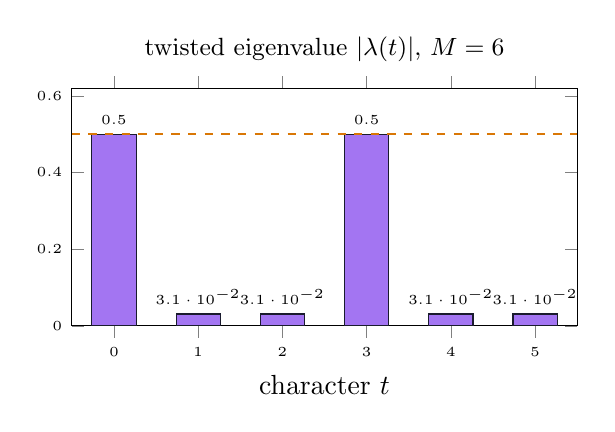
\begin{tikzpicture}\begin{axis}[width=8cm,height=4.6cm,ybar,bar width=16pt,title={\small twisted eigenvalue $|\lambda(t)|$, $M=6$},xlabel={character $t$},ymin=0,ymax=0.62,xtick={0,1,2,3,4,5},tick label style={font=\tiny},nodes near coords,every node near coord/.append style={font=\tiny}]
\addplot[draw=ink,fill=acc!70] coordinates{(0,0.5) (1,0.031) (2,0.031) (3,0.5) (4,0.031) (5,0.031)};
\draw[amb,thick,dashed](axis cs:-0.5,0.5)--(axis cs:5.5,0.5) node[right,font=\tiny]{};\end{axis}\end{tikzpicture}\end{center}
\noindent The consequence: the offset equidistributes. Mod $5$, the five residues occur with frequencies $0.199, 0.200, 0.202, 0.200, 0.199$ --- uniform to a fraction of a percent.

\section{The uniform gap --- and the open lemma}
For each \emph{fixed} $M$ the contraction is rigorous (finite-extension spectral-gap theory over the mixing base). The subtlety is that detecting $\{1,3,5\}$ exactly forces the modulus $M$ to \emph{grow with the scale}. The plot below sweeps the character frequency $\xi=t/M$ across the band: the profile is flat and small, capped near $\lead{0.082}$, with no spike toward $1$ --- \emph{no resonance}.

\begin{center}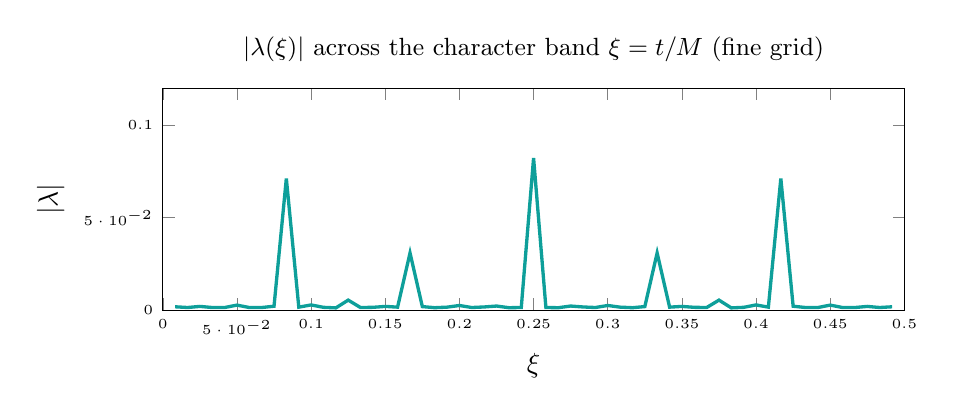
\begin{tikzpicture}\begin{axis}[width=11cm,height=4.4cm,title={\small $|\lambda(\xi)|$ across the character band $\xi=t/M$ (fine grid)},xlabel={$\xi$},ylabel={$|\lambda|$},ymin=0,ymax=0.12,xmin=0,xmax=0.5,tick label style={font=\tiny}]
\addplot[tea,very thick] coordinates{(0.0083,0.0018) (0.0167,0.0014) (0.025,0.002) (0.0333,0.0014) (0.0417,0.0014) (0.05,0.0027) (0.0583,0.0014) (0.0667,0.0014) (0.075,0.0021) (0.0833,0.0712) (0.0917,0.0016) (0.1,0.0028) (0.1083,0.0015) (0.1167,0.0012) (0.125,0.0054) (0.1333,0.0014) (0.1417,0.0015) (0.15,0.002) (0.1583,0.0016) (0.1667,0.0309) (0.175,0.0019) (0.1833,0.0013) (0.1917,0.0016) (0.2,0.0025) (0.2083,0.0014) (0.2167,0.0017) (0.225,0.0022) (0.2333,0.0013) (0.2417,0.0014) (0.25,0.0822) (0.2583,0.0014) (0.2667,0.0013) (0.275,0.0022) (0.2833,0.0017) (0.2917,0.0014) (0.3,0.0025) (0.3083,0.0016) (0.3167,0.0013) (0.325,0.0019) (0.3333,0.0309) (0.3417,0.0016) (0.35,0.002) (0.3583,0.0015) (0.3667,0.0014) (0.375,0.0054) (0.3833,0.0012) (0.3917,0.0015) (0.4,0.0028) (0.4083,0.0016) (0.4167,0.0712) (0.425,0.0021) (0.4333,0.0014) (0.4417,0.0014) (0.45,0.0027) (0.4583,0.0014) (0.4667,0.0014) (0.475,0.002) (0.4833,0.0014) (0.4917,0.0018)};\end{axis}\end{tikzpicture}\end{center}

The twisted Lasota--Yorke inequality has a variation constant that grows like $(1+|t|)$; beating that as $M\to\infty$ --- turning ``no resonance'' into a \emph{uniform} gap --- is a \lead{Dolgopyat oscillatory-cancellation estimate}. Our operator sits outside the settled theory on two counts: the cost is a multiplicative coordinate (not a Birkhoff sum, so Baladi--Vall\'ee does not apply), and the branch matrices have determinant $\pm3$ (non-unimodular, so homogeneous-dynamics is out). This one lemma is stated precisely and \emph{not} proved; it is the honest frontier.

\vspace{4pt}\hrule\vspace{4pt}\noindent{\small\color{gray} What is proved: the twisted Lasota--Yorke inequality and fixed-$M$ equidistribution. What is open: the modulus-uniform gap. The numerics establish that the gap is not blocked by a resonance --- not that it is uniform.}
\end{document}